Dans cette section, nous allons présenter les hypothèses que nous avons posé et nous présenterons notre analyse du nombre de vulnérabilités communes entre les logiciels.

\subsection{Hypothèses de base}\label{sec:hypothese}
Nous allons maintenant présenter les différentes hypothèses que nous faisons pour définir notre modèle.
Dans un premier temps, nous parlerons de l'environnement que nous considérons.
Puis dans une deuxième partie, nous discuterons des capacités que possèdent aussi bien l'attaquant que le défenseur.
Finalement nous poserons les objectifs de chacune des parties.

\subsubsection{Environnement}\label{sec:hypothese:env}
Dans le cadre de cette étude, nous considérons un environnement $E$ composé de $m$ machines utilisant une même application.
Une application représente la fonctionnalité d'un logiciel.
Il y a jusqu'à $n$ logiciel pour une application donnée.
Pour chacun de ces logiciels, nous considérons que le nombre de vulnérabilités augmente avec le temps.
Nous posons également comme hypothèse qu'il n'y a pas de vulnérabilité zero-day exploitable.
Finalement, aucun des logiciels ne possède de vulnérabilité commune.


\subsubsection{Capacité des parties}\label{sec:hypothese:capacite}
Dans le cadre de cette étude et afin de pouvoir étudier l'impact de l'hétérogénéité,  nous considérons que le défenseur ne possède
pas de système de protection contre les logiciels malveillants.
Cependant nous supposons qu'il est capable de déployer une mise à jours d'un logiciel sur toutes les machines du système en même temps.

Pour l'attaquant, nous supposons qu'il possède uniquement un malware et que celui-ci n'exploite qu'une seule vulnérabilité.
Le malware ne peut donc cibler qu'un seul logiciel.
Cela nous permet de montrer l'impact maximal sur le système.


\subsubsection{Les objectifs des parties}\label{sec:hypothese:objectifs}
Pour pouvoir étudier l'efficacité du système hétérogène, nous supposons que l'objectif de l'attaquant est de propager un malware
et d'infecter le plus de machines possible.
Pour le défenseur l'objectif est d'assurer que le système reste disponible.


%\begin{figure}
%\centering
%%peut être la faire avec des exemple de vulnérabilité réelles
%\begin{tikzpicture}[->,>=stealth',shorten >=1pt,auto,node distance=1cm,
%  thick,version node/.style={circle,fill=blue!15,draw,
%  font=\sffamily\small\bfseries,minimum size=5mm}, vulne node/.style={circle,fill=red!15,draw,
%  font=\sffamily\small\bfseries,minimum size=5mm}]
%  
%  \node[version node] (L0) {L1};
%  \node[version node] (L1) [below of=L0] {L2};
%  \node[version node] (L2) [below of=L1] {L3};
%  \node[version node] (L3) [below of=L2] {L4};
%  \node[version node] (L4) [below of=L3] {L5};
%  
%  \node[vulne node] (V1) [right of=L0, node distance=3cm] {V1};
%  \node[vulne node] (V2) [below of=V1] {V2};
%  \node[vulne node] (V3) [below of=V2] {V3};
%  \node[vulne node] (V4) [below of=V3] {V4};
%  \node[vulne node] (V5) [below of=V4] {V5};
%
%%connexion vulnerabilité 1
%  \draw [-latex'] (V1) -- (L0);
%  \draw [-latex'] (V1) -- (L1);
%  \draw [-latex'] (V1) -- (L2);
%  \draw [-latex'] (V1) -- (L4);
%  
%%connexion vulnerabilité 2
%  \draw [-latex'] (V2) -- (L0);
%  \draw [-latex'] (V2) -- (L1);
%  \draw [-latex'] (V2) -- (L2);
%
%%connexion vulnerabilité 3
%  \draw [-latex'] (V3) -- (L0);
%  \draw [-latex'] (V3) -- (L2);
%
%%connexion vulnerabilité 4
%%  \draw [-latex'] (V4) -- (L4);
%  \draw [-latex'] (V4) -- (L2);
%  \draw [-latex'] (V4) -- (L3);
%
%%connexion vulnerabilité 5
%  \draw [-latex'] (V5) -- (L4);
% 
%  
%\end{tikzpicture}
%\caption{Schéma de la relation entre la version d'un logiciel et les vulnérabilités associées.}
%\label{fig:heteImpactVuln}
%\end{figure}

%Pour analyser cette impact, nous considérons deux éléments, le nombre total $T$ de vulnérabilités du système ainsi que le nombre minimum $M$ de vulnérabilités nécessaires pour contaminer entièrement le système.
%$T$ permet d'estimer la probabilité qu'un attaquant possède un exploit, plus ce nombre est élevé et plus la probabilité est grande.
%$M$ permet d'estimer la complexité pour l'attaquant s'il veut attaquer tout les ordinateurs du système.
%Plus ce nombre est élevé, plus la difficulté est importante.
%
%\paragraph{L'impact des mises à jours}
%Dans le paragraphe précédent, nous avons expliqué l'intérêt qu'il y a à la diversité des versions.
%Toutefois, nous n'avons pas pris en compte l'ancienneté d'une vulnérabilité. 
%L'ancienneté d'une vulnérabilité la rend plus facilement exploitable car plus connue.
%De plus, comme expliqué dans la section~\ref{sec:modelMath}, le fait de faire des mises à jours forcera l'attaquant à augmenter l'effort pour être capable de s'adapter à ce changement.
%
%Pour évaluer l'impact de l'ancienneté d'une version, nous ajoutons une majoration à la probabilité que l'attaquant possède une vulnérabilité.
%En effet, il est peu probable qu'un attaquant possède un exploit pour une vulnérabilité récente alors qu'il est bien plus facile pour lui d'en obtenir un pour une ancienne vulnérabilité.
%Finalement, nous sommes capable d'estimer l'effort nécessaire pour un attaquant pour déterminer les différentes versions de logiciel utilisées lors d'une mise à jour.



%\paragraph{L'impact de l'hétérogénéité du système}
%Le fait d'avoir un système hétérogène amène à une augmentation du nombre total de vulnérabilités.
%Cependant cette diversité peut rendre une attaque globale plus complexe vue que chacun des systèmes sera sensible à des attaques différentes.
%La figure~\ref{fig:heteImpactVuln} exprime cette notion de non concordance entre les vulnérabilités et leur version.
%Dans cette figure, les nœuds "Ln" représentent une version de logiciel et les nœuds "Vn" représentent un numéro de vulnérabilité.
%Nous voyons que certaines versions n'ont aucune vulnérabilité commune avec d'autre tel que "L4" avec et "L5".
%Dans ce cas, il est plus compliqué d'attaquer les deux systèmes simultanément.
%Cependant, si nous prenons le cas de "L1" et "L2", ils sont tout deux sensibles à "V1" et "V2".
%Dans ce cas, la diversité amène une augmentation du risque d'attaques.


\subsection{Analyse du nombre de vulnérabilités par logiciel}
Nous avons extrait depuis la base de données de vulnérabilité du gouvernement américain NVD~\cite{vulnDatabase} le nombre de failles par logiciel.
Cette base de donnée contient une liste des vulnérabilités connues.
La figure~\ref{fig:vulPerLog} montre le nombre de vulnérabilité communes à au moins deux logiciels sur les 70285 vulnérabilités connues.
Il est également nécessaire de considérer que certains logiciels ont des identifications différentes mais sont les mêmes.
Nous avons un total de 4,70\% de logiciels ayant des vulnérabilités communes donc 73\% concerne uniquement 2 logiciels.
Nous pouvons donc considérer que notre hypothèse sur le fait qu'il n'y ait pas de vulnérabilités communes entre plusieurs
logiciels est correcte. En effet, le nombre de logiciels présents dans cette base de données nous paraît suffisamment grand pour
être représentatif.

\begin{figure}
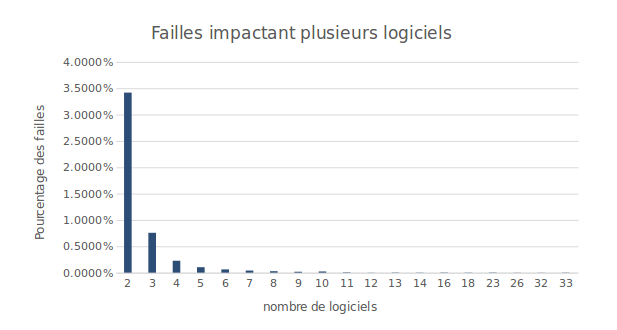
\includegraphics[width=\linewidth]{data/commonVuln.png}
\caption{Compte des vulnérabilités communes à au moins 2 logiciels sur les 70285 vulnérabilités connues.}
\label{fig:vulPerLog}
\end{figure}

